%! TeX program = xelatex
\documentclass[10pt]{beamer}
\usepackage{adjustbox}
\usepackage{graphicx}
\usepackage{algorithm}
\usepackage{algpseudocode}
\usepackage{amsmath}
\usepackage{subcaption}
\usepackage{multirow}
\usepackage{amsmath}
\usepackage{siunitx}
\usepackage{booktabs}
\usepackage{caption}
\usepackage{array}
\usepackage[dvipsnames,table]{xcolor}
\usepackage{fontspec}
\usepackage{BeamerCobaltDarkTheme}

% Custom colors
\definecolor{primary}{RGB}{0, 164, 254}

\title{Statistical Analysis of Experimental Results\\
The Tournament}
\author{Brandon Marquez Salazar}
\institute{Curso de Estadística Inferencial}
\date{}

\begin{document}

% Title page with custom background
{
\setbeamertemplate{background}{%

\includegraphics[width=\paperwidth, height=\paperheight]{fondo.png}
}

\begin{frame}
\titlepage
\end{frame}
}

{
   \setbeamertemplate{background}{%
   
\includegraphics[width=\paperwidth, height=\paperheight]{blured.png}
   }
   
   \begin{frame}{Normality Test Results - Shapiro-Wilk Test}
   \centering
   \begin{tabular}{l S[table-format=1.6] S[table-format=1.6] c}
   \toprule
   \textbf{Dataset} & \textbf{Statistic (W)} & \textbf{P-value} & \textbf{Normal} \\
   \midrule
   Dataset de Brandon & 0.996800 & 0.955533 & True \\
   Dataset de Cindy & 0.983705 & 0.020487 & False \\
   \bottomrule
   \end{tabular}
   \captionof{table}{Shapiro-Wilk normality test results. Null hypothesis (H₀): Data follows a normal distribution.}
   \end{frame}

   \begin{frame}{Normality Test Results}
      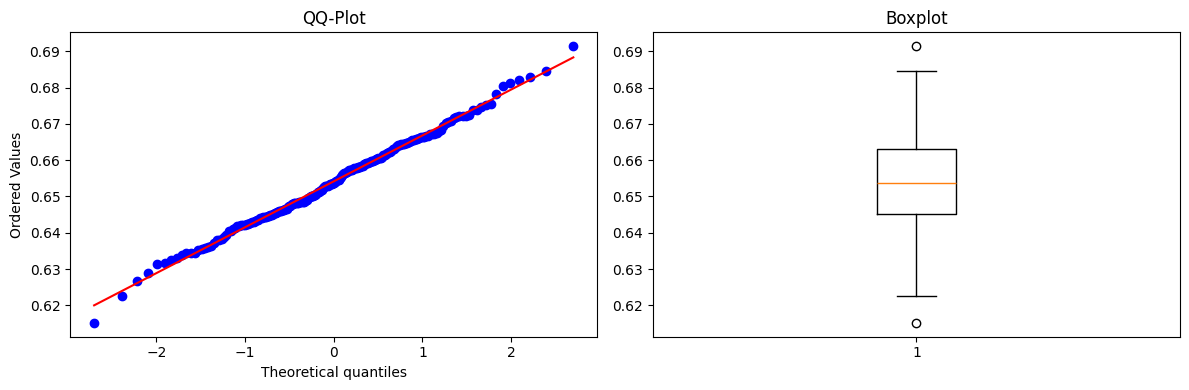
\includegraphics[width=\textwidth]{normality_plots_Dataset de Brandon.png} 
      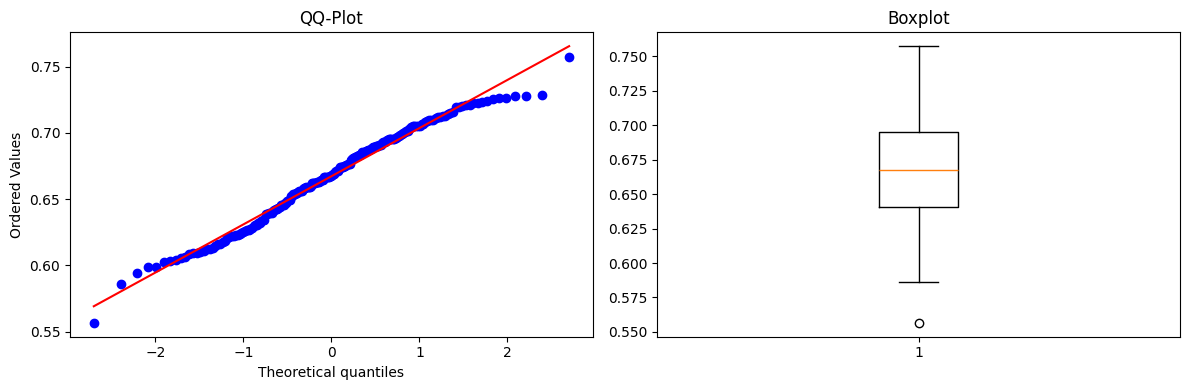
\includegraphics[width=\textwidth]{normality_plots_Dataset de Cindy.png} 
   \end{frame}

   \begin{frame}{Dataset Overview - Descriptive Statistics}
   \centering
   \scriptsize
   \begin{tabular}{l S[table-format=3.0] S[table-format=1.6] S[table-format=1.6] S[table-format=1.6]}
   \toprule
   \textbf{Dataset} & \textbf{Samples} & \textbf{Mean} & \textbf{Median} & \textbf{Std} \\
   \midrule
   Dataset de Brandon & 200 & 0.654155 & 0.653683 & 0.012535 \\
   Dataset de Cindy & 200 & 0.667328 & 0.667888 & 0.036239 \\
   \bottomrule
   \end{tabular}
   
   \vspace{0.5cm}
   \begin{tabular}{l S[table-format=1.6] S[table-format=1.6]}
   \toprule
   \textbf{Dataset} & \textbf{Minimum} & \textbf{Maximum} \\
   \midrule
   Dataset de Brandon & 0.615156 & 0.691413 \\
   Dataset de Cindy & 0.556569 & 0.757423 \\
   \bottomrule
   \end{tabular}
   \captionof{table}{Descriptive statistics for both datasets showing central tendency and dispersion measures.}
   \end{frame}

   \begin{frame}{Variance Test - Levene Test Results}
   \centering
   \begin{tabular}{l S[table-format=3.6] S[table-format=1.6e1] c}
   \toprule
   \textbf{Method} & \textbf{Statistic} & \textbf{P-value} & \textbf{Equal Variance} \\
   \midrule
   Levene & 167.485723 & 3.222765e-32 & False \\
   \bottomrule
   \end{tabular}
   \captionof{table}{Levene test for equality of variances between datasets. The extremely small p-value indicates significant difference in variances.}
   \end{frame}

   \begin{frame}{Statistical Difference Test - Wilcoxon Rank-Sum Test}
   \centering
   \begin{tabular}{l S[table-format=5.1] S[table-format=1.6e1] c}
   \toprule
   \textbf{Method} & \textbf{Statistic} & \textbf{P-value} & \textbf{Equal Distributions} \\
   \midrule
   Wilcoxon & 14466.0 & 1.699915e-06 & False \\
   \bottomrule
   \end{tabular}
   \captionof{table}{Wilcoxon rank-sum test results. The small p-value indicates statistically significant difference between the two datasets.}
   \end{frame}

   \begin{frame}{Complete Statistical Analysis Summary}
   \centering
   \scriptsize
   \begin{tabular}{l l l l l}
   \toprule
   \textbf{Test Type} & \textbf{Dataset 1 Result} & \textbf{Dataset 2 Result} & \textbf{Test Statistic} & \textbf{Conclusion} \\
   \midrule
   Normality (Shapiro-Wilk) & Normal (p=0.9555) & Not Normal (p=0.0205) & W=0.9968/0.9837 & Mixed normality \\
   Variance (Levene) & \multicolumn{2}{l}{Variances not equal} & F=167.49 & Heteroscedastic \\
   Difference (Wilcoxon) & \multicolumn{2}{l}{Distributions different} & W=14466.0 & Statistically different \\
   \bottomrule
   \end{tabular}
   
   \vspace{0.5cm}
   \begin{block}{Key Findings}
   \begin{itemize}
   \item Dataset de Brandon follows normal distribution
   \item Dataset de Cindy does not follow normal distribution  
   \item Variances between datasets are significantly different
   \item The two datasets show statistically significant differences
   \item Non-parametric Wilcoxon test was appropriate due to violated assumptions
   \end{itemize}
   \end{block}
   \end{frame}

   \begin{frame}{Statistical Analysis Pseudocode - Main Functions}
   \scriptsize
   \begin{algorithmic}[1]
   \Function{statistical\_analysis}{opts}
      \State res["normality\_test"][opts.ds\_01\_name] $\gets$ Normality\_Test(opts.ds\_01)
      \State res["overview"][opts.ds\_01\_name] $\gets$ DatasetOverview(opts.ds\_01)
      \If{ds\_02 exists}
         \State res["normality\_test"][opts.ds\_02\_name] $\gets$ Normality\_Test(opts.ds\_02)
         \State res["overview"][opts.ds\_02\_name] $\gets$ DatasetOverview(opts.ds\_02)
         \State res["variance\_test"] $\gets$ Variance\_Test(opts, res)
         \State res["difference\_test"] $\gets$ Statistical\_Difference\_Test(opts, res)
      \EndIf
      \State \Return res
   \EndFunction
   
   \Function{Normality\_Test}{ds}
      \State out $\gets$ Shapiro-Wilk(ds)
      \State out["method"] $\gets$ "Shapiro-Wilk"
      \If{out["p-value"] $<$ 0.05}
         \State out["normal"] $\gets$ false
      \Else
         \State out["normal"] $\gets$ true
      \EndIf
      \State \Return out
   \EndFunction
   \end{algorithmic}
   \end{frame}

   \begin{frame}{Statistical Analysis Pseudocode - Support Functions}
   \scriptsize
   \begin{algorithmic}[1]
   \Function{DatasetOverview}{ds}
      \State out["samples"] $\gets$ length(ds)
      \State out["mean"] $\gets$ mean(ds)
      \State out["median"] $\gets$ median(ds)
      \State \Return out
   \EndFunction
   
   \Function{Variance\_Test}{opts, res}
      \If{both datasets normal}
         \State out $\gets$ F-Test(opts.ds\_01, opts.ds\_02)
         \State out["method"] $\gets$ "F-Test"
      \Else
         \State out $\gets$ Levene(opts.ds\_01, opts.ds\_02)
         \State out["method"] $\gets$ "Levene"
      \EndIf
      \If{out["p-value"] $<$ 0.05}
         \State out["equal"] $\gets$ false
      \Else
         \State out["equal"] $\gets$ true
      \EndIf
      \State \Return out
   \EndFunction
   \end{algorithmic}
   \end{frame}

   \begin{frame}{Statistical Analysis Pseudocode - Difference Test}
   \scriptsize
   \begin{algorithmic}[1]
   \Function{Statistical\_Difference\_Test}{opts, res}
      \If{both normal and equal variance}
         \State out["alpha\_grid"] $\gets$ alpha\_optimizer(opts.ds\_01, opts.ds\_02, opts)
         \State out $\gets$ T-Test(opts.ds\_01, opts.ds\_02, best\_alpha)
         \State out["method"] $\gets$ "T-Test"
         \If{out["p-value"] $<$ best\_alpha}
            \State out["equal"] $\gets$ false
         \Else
            \State out["equal"] $\gets$ true
         \EndIf
      \Else
         \State out $\gets$ Wilcoxon(opts.ds\_01, opts.ds\_02)
         \State out["method"] $\gets$ "Wilcoxon"
      \EndIf
      \State \Return out
   \EndFunction
   \end{algorithmic}
   \end{frame}

   \begin{frame}{Statistical Analysis Pseudocode - Alpha Optimizer}
   \scriptsize
   \begin{algorithmic}[1]
   \Function{alpha\_optimizer}{x, y, opts}
      \State alpha\_list $\gets$ opts["alpha"]["values"] or default
      \State P $\gets$ opts["alpha"]["P"] or 0.4
      \State k $\gets$ opts["alpha"]["k"] or 1
      \State sample\_size $\gets$ opts["alpha"]["sample\_size"] or 6
      \State iterations $\gets$ opts["alpha"]["iterations"] or 500
      
      \For{each alpha in alpha\_list}
         \For{i in 1 to iterations}
            \State sample\_x $\gets$ sample(x, sample\_size, replace=True)
            \State sample\_y $\gets$ sample(y, sample\_size, replace=True)
            \State pvalue $\gets$ t.test(sample\_x, sample\_y)\$p.value
            \State update rejection\_count
         \EndFor
         \State power $\gets$ rejected / total
         \State beta $\gets$ 1 - power
         \State expected\_loss $\gets$ (P * alpha) + ((1 - P) * k * beta)
      \EndFor
      \State best\_alpha $\gets$ alpha with min(expected\_loss)
      \State \Return results with best\_alpha
   \EndFunction
   \end{algorithmic}
   \end{frame}
}

\end{document}
